\section{Implementation, integration and test plan}
The eMall will be naturally divided as follows:
\begin{itemize}
    \item eMsp: Application Server
    \item eMsp: Mobile App
    \item CPO: Application Server
    \item CPO: WebServer
\end{itemize}
The implementation logic will be Bottom up. In this way the integration testing will follow the implementation and less code will be required as stubs are not necessary.\\
All these macro-components can be developed in a parallel manner, but the main focus will be on the Application servers for both the CPO and the eMSP, as they are the most difficult and complex parts.\\
The building and the integration will be strongly related, so the integration and testing plans will strictly follow the implementation's one.\\
In the following table a mapping between functionalities, importance for the customer and implementation difficulty is carried on, so that we can better plan the module implementation order:\\

\begin{center}
    \begin{table}[H]
        \makebox[\linewidth]{
        \begin{tabular}{ | c |c | c | c |}
            \hline
            \textbf{Functionality} & \textbf{Module} & \textbf{Importance for customer} & \textbf{Difficulty} \\ \hline
            Sign Up and Login                               & eMSP          & High      & Low                 \\ \hline
            View the nearby charging stations               & eMSP-CPMS          & High      & Medium              \\\hline
            Charge booking                                  & eMSP-CPMS          & Medium    & High                \\\hline
            Remotely unlocking a socket                     & eMSP-CPMS          & Medium    & Medium              \\\hline
            Remotely starting a charge                      & eMSP-CPMS          & Medium    & Medium                \\\hline
            Notify of a finished charge                     & eMSP-CPMS          & Low       & Medium                \\\hline
            Pay for the service                             & eMSP          & Medium    & High                \\\hline
            Change active vehicle for the suggestions       & eMSP          & Low       & High                \\\hline
            Select the charging station’s energy provider   & CPMS           & High      & High                \\\hline
            Select a battery policy for a charging station  & CPMS           & High      & High                \\\hline
            Select the charging station’s charging cost     & CPMS           & High      & High                \\

            \hline
        \end{tabular}
        }
        \caption{functionalities importance - difficulty mapping}\label{implementation_precedences}
    \end{table}
\end{center}



As the importance of functionalities for the customer is mainly Medium-High, and considering that most of the functionalities are necessary for the correct working of the application, the implementation order will not follow the "Importance for the customer" factor. The implementation order will follow the bottom up structure of the modules. Firstly the CPMS module will be developed, and then the eMSP as the eMSP strongly depends on the CPMS.\\

All the modules rely on the DBMSs, so this component must be the first one to be implemented.
The following picture describes the implemetnation schedule of the main components of the CPMS and eMSP application servers:
% TODO CENTER THIS IMAGE!!
\begin{center}
    \begin{figure}[H]
        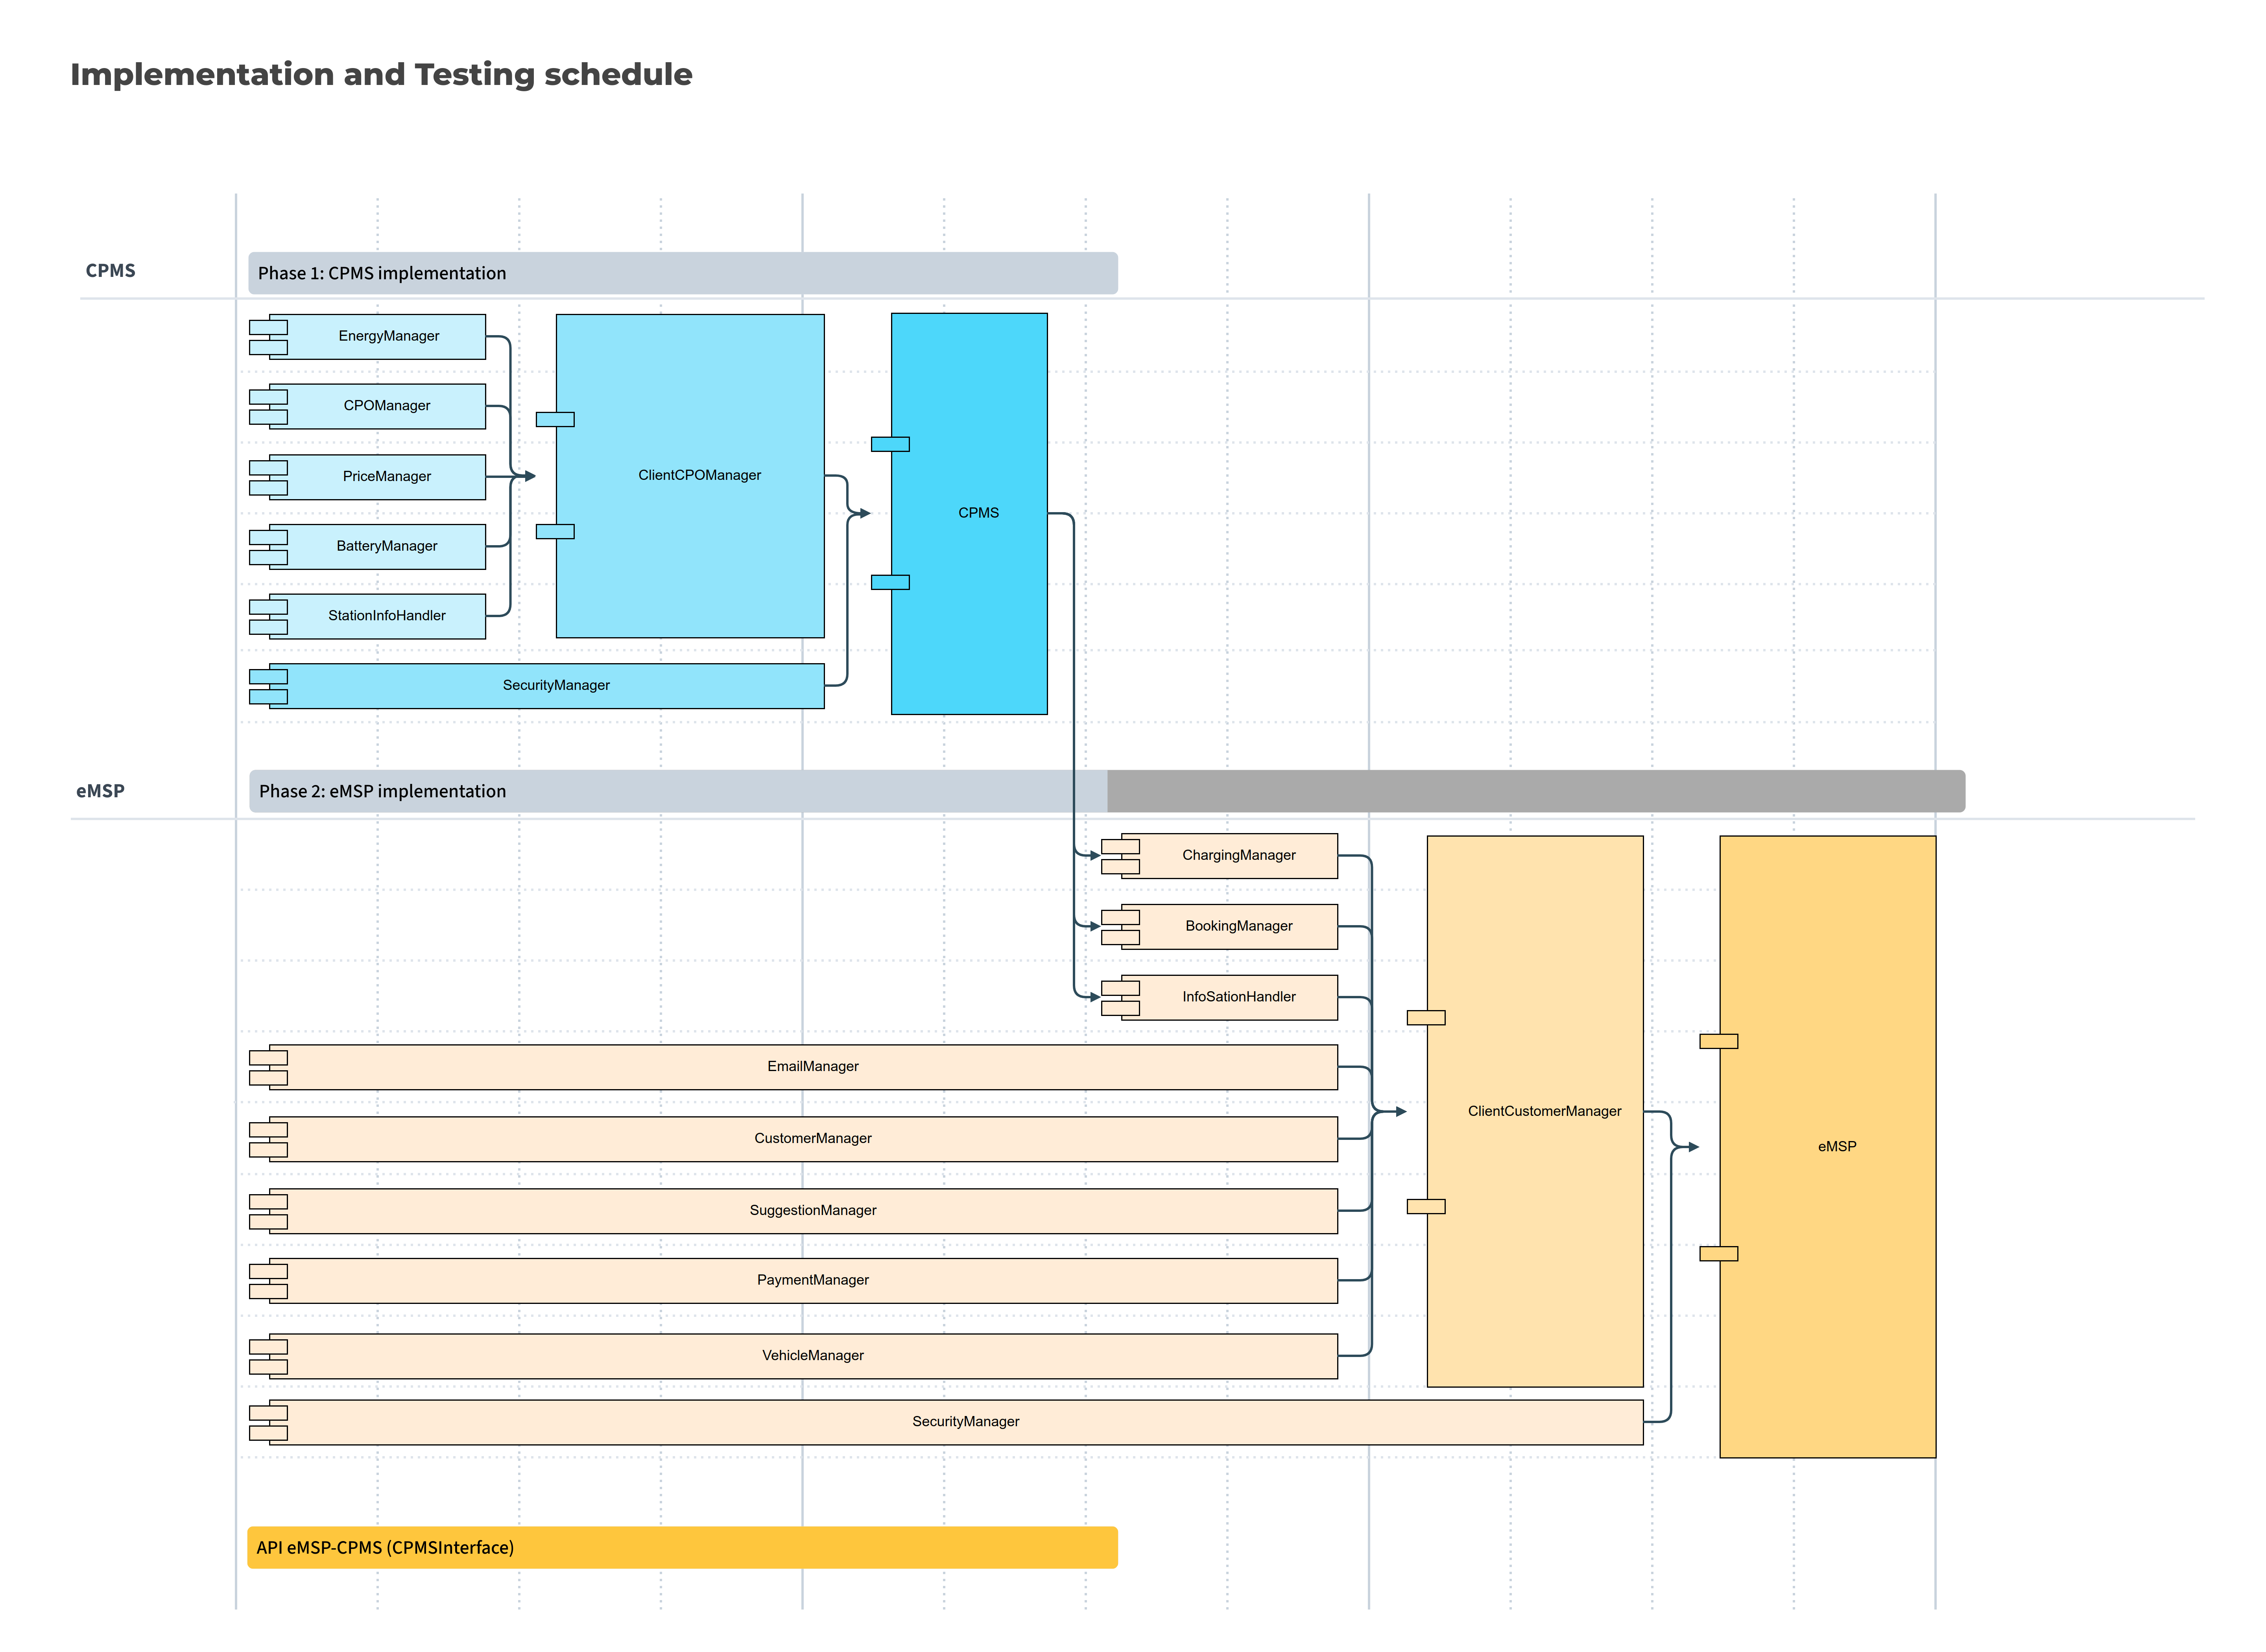
\includegraphics[width=\textwidth]{./img/ImplementationOrder.png}
        \caption{Implementation schedule of the main components of the CPMS and eMSP application servers, arrows represent precedence operator}
    \end{figure}
\end{center}

The first subsystem to be developed is the CPMS, it's internal modules can be implemented in parallel. For each one of them unit testing must be carried out, the integration testing is done with the DBMS and the ExternalAPIs. After that, is composed the ClientCPOManager and the CPMS Application server, for both of them as soon as they are implemented unit testing is made, while integration testing will be done when the eMSP and or the WebServer will be implemented. \\

In the mean-while components of the eMSP Application server that are not related with the CPMS can be implemented and tested, both doing unit testing and integration testing with the DBMS, the PaymentAPI and the VehicleAPI.\\

The development of the communication API between CPMS and eMSP (CPMSInterface) can be carried out in parallel, it must be completed in order to develop and test the remaining modules of the eMSP.\\

Once the CPMS and the CPMSInterface are ready, the remaining components of the eMSP Application server are implemented. For them unit testing and integration testing are carried out. The integration testing uses the CPMSInterface to verify the correct operating functionalities.\\

When the two application server are fully implemented integration testing between them is done, a driver will test using their interfaces, their functionalities.\\

The eMSP's mobile app and the CPO's WebServer can be developed in parallel to the application servers.\\
Once the CPO's WebServer is ready,it is performed integration testing with the CPMS's Application Server to verify the overall CPMS system functionality..
Once the eMSP's mobile app is ready it is performed integration testing with the eMSP's Application Server to verify the overall eMSP system functionality.\\
If both the CPO's and the eMSP's subsytems are fully working the overall system is functioning properly.


It's not specified each specific unit tests, but the coverage must be of at least 80\% of code lines.
